\chapter{Particle Simulator}
\label{chap:particle-simulator}

\input{chapters/out/Particle Simulator.md.tex}
\input{chapters/out/Leapfrog Integration.md.tex}

\begin{figure}[H]
  \centering
  \label{fig:gui-screenshot}
  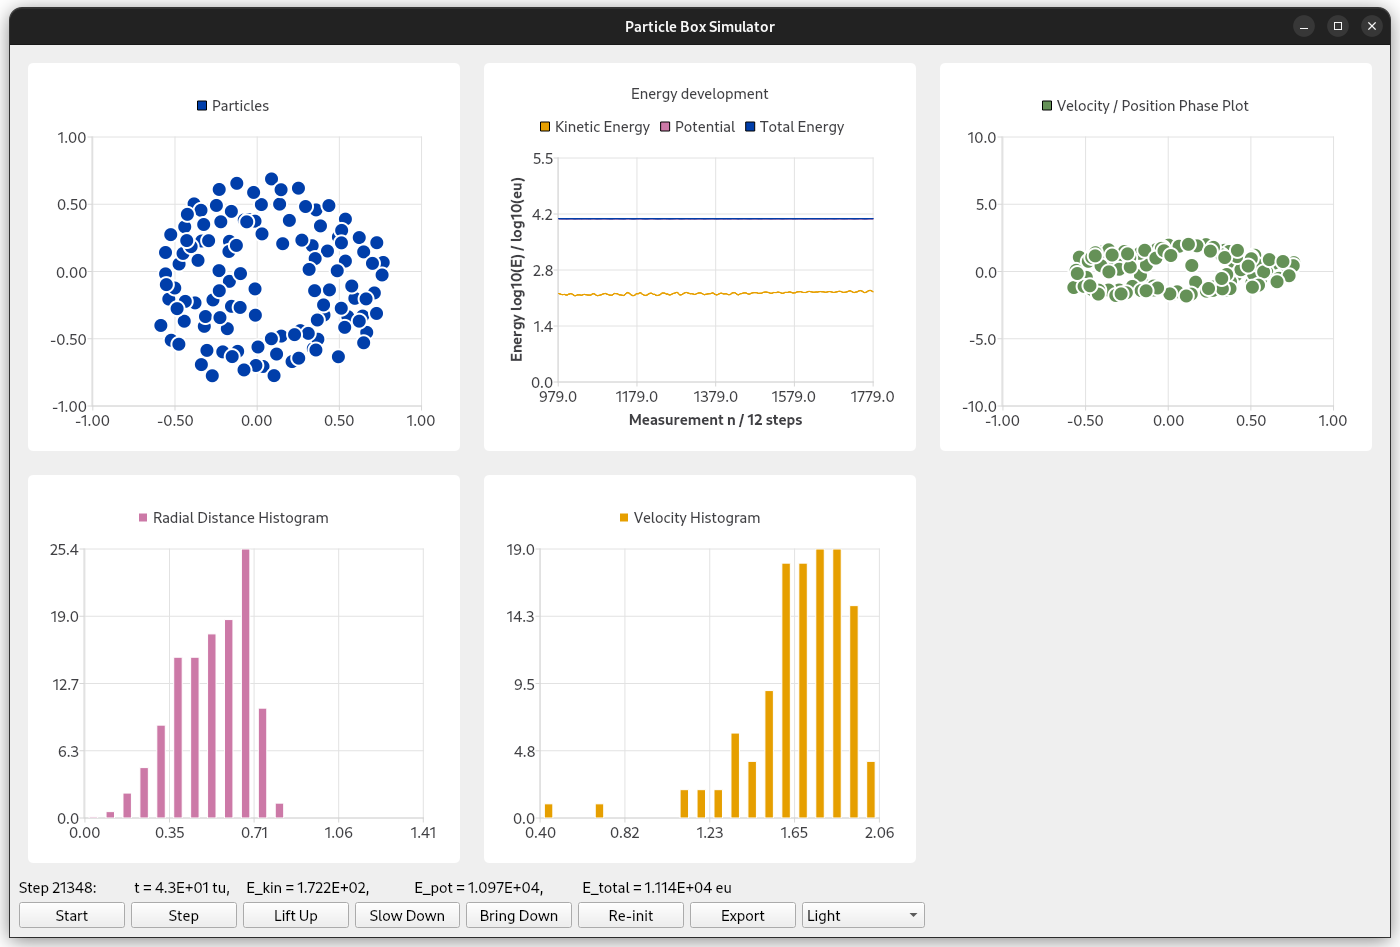
\includegraphics[width=\linewidth]{gui-screenshot.png}
  \caption{Screenshot of the GUI}
\end{figure}

\begin{figure}[H]
  \centering
  \label{fig:simulation-quiver}
  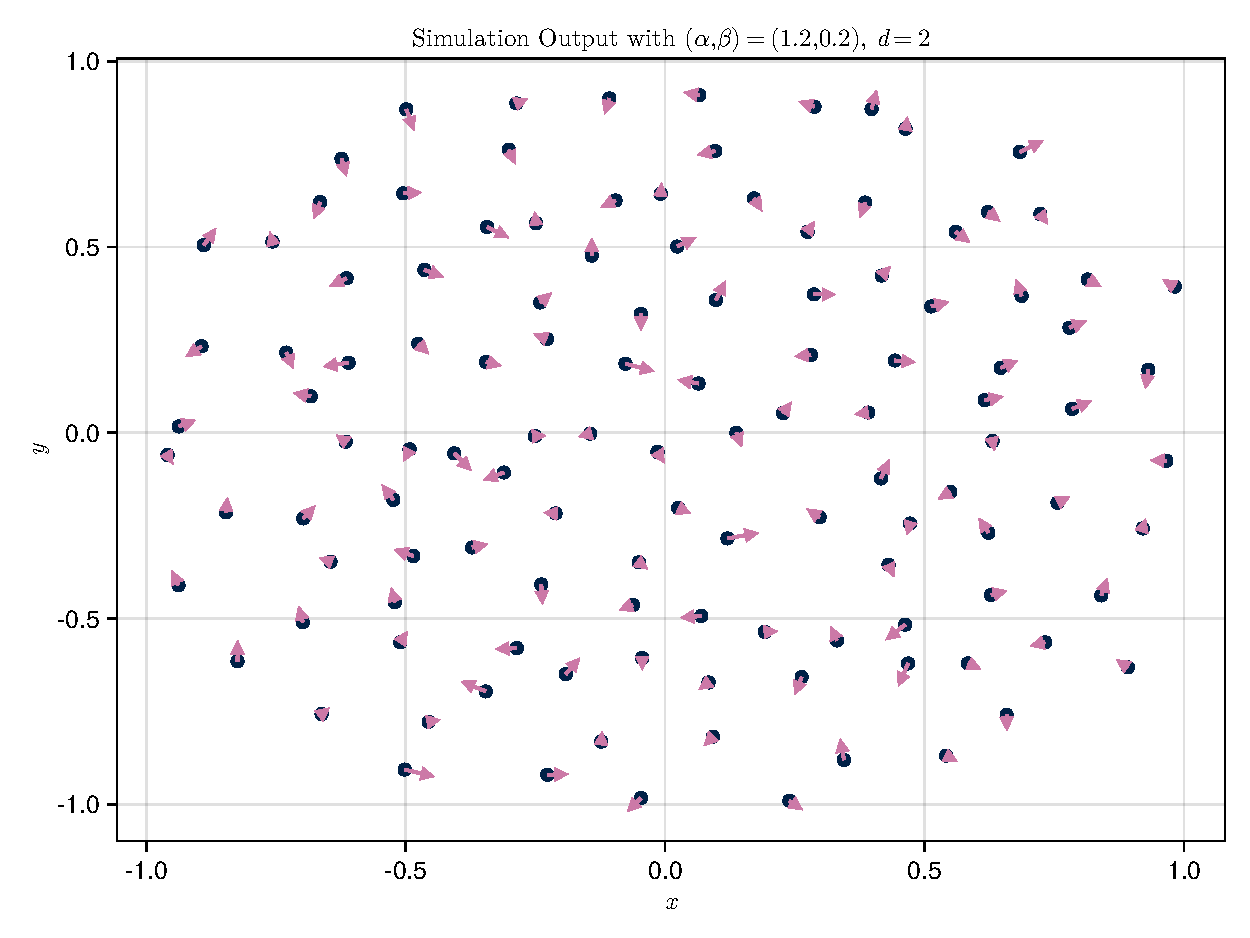
\includegraphics[width=0.8\linewidth]{results/simulation-quiver.pdf}
  \caption{Position and velocity of particles in the simulation.}
\end{figure}

\begin{figure}[H]
  \centering
  \label{fig:phase-space-plot}
  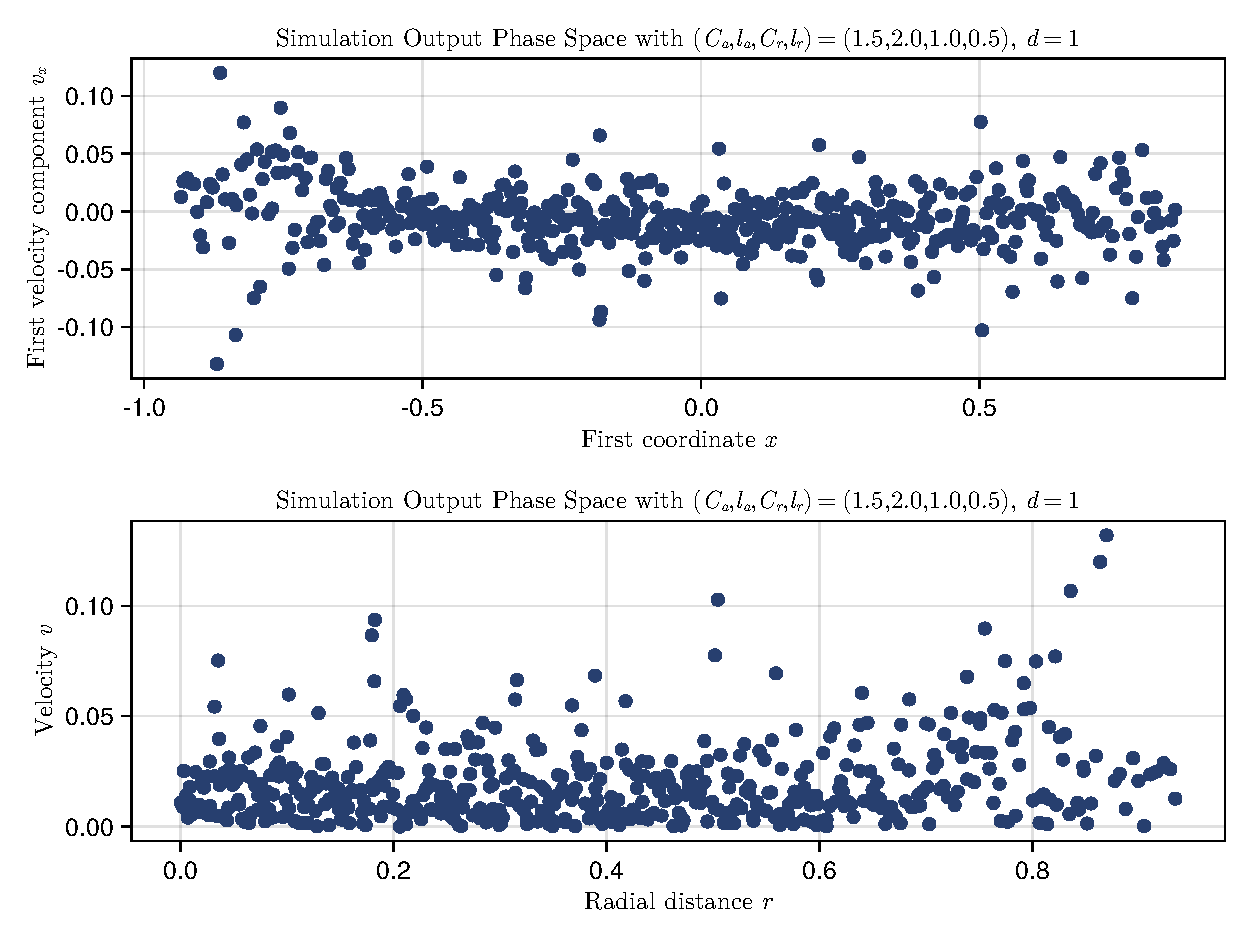
\includegraphics[width=0.8\linewidth]{results/phase-space-plot.pdf}
  \caption{Position and velocity of particles in the simulation visualised as a phase space plot.}
\end{figure}

\begin{figure}[H]
  \centering
  \label{fig:simulation-histogram}
  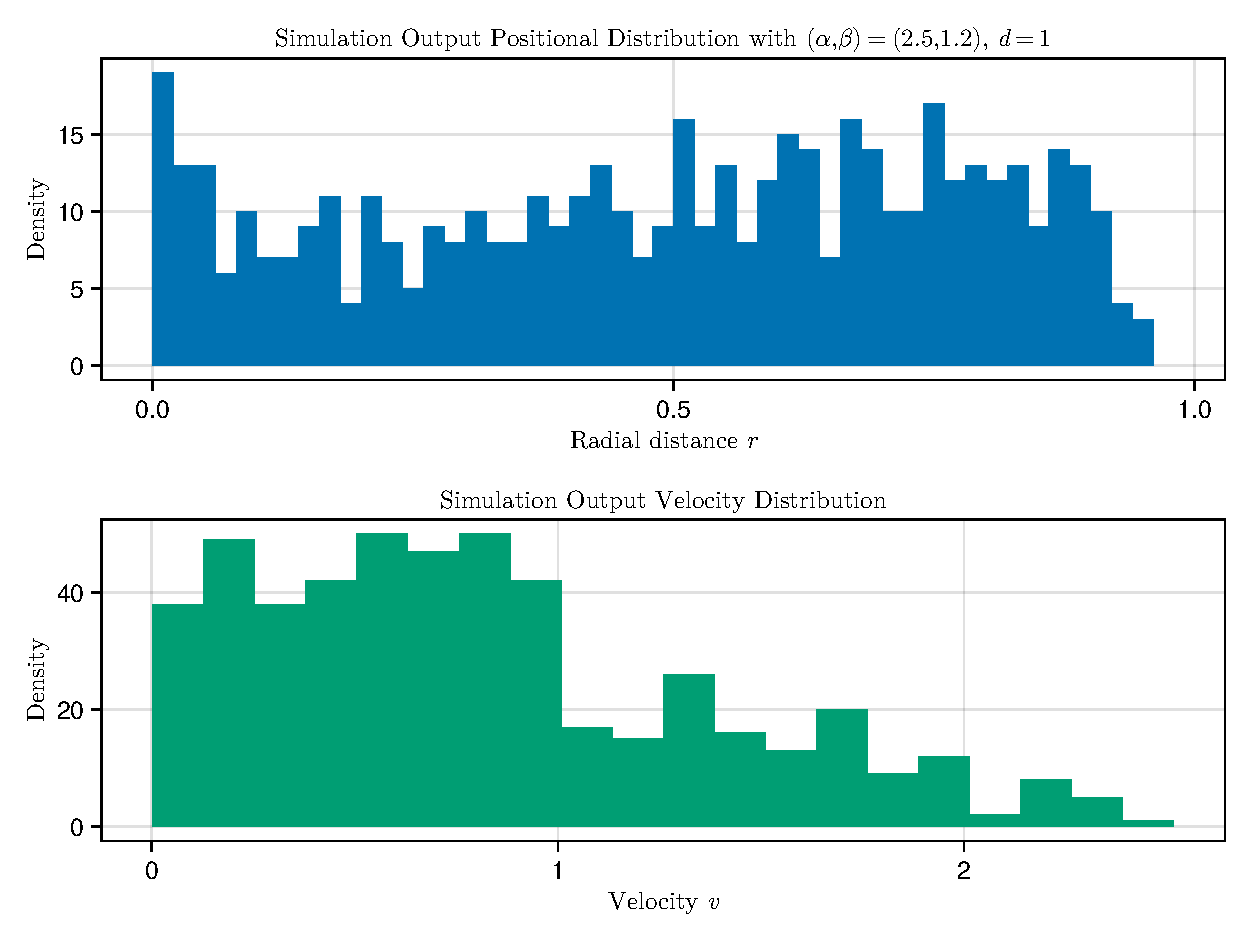
\includegraphics[width=0.8\linewidth]{results/simulation-histogram.pdf}
  \caption{Position Histogram}
\end{figure}
